\chapter{Metode Penelitian}

\section{Alat dan Bahan Tugas akhir}

\subsection{Alat Tugas akhir}

Pengerjaan penelitian ini menggunakan alat dan bahan. alat yang digunakan berupa perangkat keras seperti laptop untuk menjalankan program, software, serta library yang 
akan digunakan.

\begin{enumerate}
	\item \textit{Laptop} dengan spesifikasi sebagai berikut :
            \begin{itemize}
                \item Sistem operasi Windows 10
                \item {Processor} Intel I7-8750H
                \item Memori 16GB DDR4
                \item NVIDIA GeForce GTX 1050 (4GB)
                \item SSD Samsung MZNLN128HAHQ 128GB
                \item HDD HGST HTS721010A9E630
            \end{itemize}  
	\item Bahasa pemrograman python 3.10.12 sebagai interpreter. Digunakan sebagai bahasa pemrograman utama.
	\item Visual Studio Code 
	\item Google Colaboratory sebagai \textit{cloud computing} yang digunakan.
	\item Numpy Library untuk melakukan perhitungan matriks pada bahasa pemrograman python. Library utama yang digunakan untuk melakukan perhitungan matriks.
\end{enumerate}


\subsection{Bahan Tugas akhir}

% \begin{table}[H]
%     \centering
%     \begin{tabular}{||p{1em}|p{3em}|p{3em}|p{4em}||}
%     \hline
%        No & Lebar & Tinggi & Kelas\\ [0.5ex]
%         \hline\hline
%         1 & 1.1 & 1.3 & lemari\\ \hline 
%         2 & 1.1 & 1.5 & lemari\\ \hline	
%         3 & 0.7 & 1.5 & lemari\\ \hline	
%         4 & 0.6 & 1.9 & lemari\\ \hline	
%         5 & 0.8 & 2 & lemari\\ \hline	
%         6 & 1.2 & 0.6 & buffet\\ \hline	
%         7 & 1.6 & 0.5 & buffet\\ \hline	
%         8 & 1.7 & 0.7 & buffet\\ \hline	
%         9 & 2.2 & 0.4 & buffet\\ \hline	
%         10 & 2.2 & 0.5 & buffet\\ \hline	
%         11 & 2.3 & 0.8 & buffet\\ \hline	
%         12 & 1.5 & 0.5 & buffet\\ \hline
%         13 & 2 & 2 & wardrobe\\ \hline
%         14 & 1.8 & 2.2 & wardrobe\\ \hline	
%         15 & 1.5 & 1.8 & wardrobe\\ \hline	
%         16 & 2.3 & 1.5 & wardrobe\\ \hline
%         \end{tabular}
%     \caption{Dataset ukuran lebar dan tinggi dari lemari, buffet, dan wardrobe}
%     \label{tab:Dataset}
% \end{table}

Dataset yang digunakan berupa data tinggi dan lebar suatu lemari, \textit{buffet}, dan \textit{wardrobe}. 
Dataset berupa data tabular dan dapat dipisahkan secara linear.  
Dataset ini bersifat \textit{dummy} namun dengan memperhatikan dengan skala aslinya.

% \begin{figure}[H]
%     \centering
%     \begin{tikzpicture}
%         \begin{axis}[
%             xlabel=Lebar,
%             ylabel=Tinggi,
%             xmin=0, xmax=2.5,
%             ymin=0, ymax=2.5,
%             width=10cm,
%             height=7cm,
%             domain=-4:4,
%             grid=both,
%             samples=100,
%             legend pos=south west,
%             axis lines=middle, % Add this line to get the axes in the middle
%         ]

%         % Adding points
%         \addplot[mark=*, color=cyan, mark size = 3] coordinates {(1.1,1.3)};
%         \addplot[mark=*, color=cyan, mark size = 3] coordinates {(1.1,1.5)};
%         \addplot[mark=*, color=cyan, mark size = 3] coordinates {(0.7,1.5)};
%         \addplot[mark=*, color=cyan, mark size = 3] coordinates {(0.6,1.9)};
%         \addplot[mark=*, color=cyan, mark size = 3] coordinates {(0.8,2)};
%         \addplot[mark=*, color=magenta, mark size = 3] coordinates {(1.2,0.6)};
%         \addplot[mark=*, color=magenta, mark size = 3] coordinates {(1.6,0.5)};
%         \addplot[mark=*, color=magenta, mark size = 3] coordinates {(1.7,0.7)};
%         \addplot[mark=*, color=magenta, mark size = 3] coordinates {(2.2,0.4)};
%         \addplot[mark=*, color=magenta, mark size = 3] coordinates {(2.2,0.5)};
%         \addplot[mark=*, color=magenta, mark size = 3] coordinates {(2.3,0.8)};
%         \addplot[mark=*, color=magenta, mark size = 3] coordinates {(1.5,0.5)};
%         \addplot[mark=*, color=yellow, mark size = 3] coordinates {(2,2)};
%         \addplot[mark=*, color=yellow, mark size = 3] coordinates {(1.8,2.2)};
%         \addplot[mark=*, color=yellow, mark size = 3] coordinates {(1.5,1.8)};
%         \addplot[mark=*, color=yellow, mark size = 3] coordinates {(2.3,1.5)};


%         % Draw frame
%         \draw[black, thick] (rel axis cs:0,0) rectangle (rel axis cs:1,1);
%         \end{axis}
%     \end{tikzpicture}
%     \caption{Grafik dari dataset pada Tabel \ref{tab:Dataset}. \textit{Cyan} adalah lemari, \textit{magenta} adalah buffet, dan kuning adalah wardrobe}
%     \label{fig:plot dataset}
% \end{figure}

% Pada Gambar \ref{fig:plot dataset} terlihat bahwa terdapat jarak diantara ketiga kelas sehingga dataset dapat dikatakan \textit{linearly separable}.

\section{Metode yang Digunakan}

Penelitian ini menggunakan pendekatan \textit{kuantitatif} untuk menganalisis pengaruh jumlah \textit{hidden layer} terhadap akurasi dan waktu komputasi pada jaringan saraf tiruan. 
Evaluasi kinerja model dilakukan dengan mengukur nilai akurasi dan waktu pelatihan, yang selanjutnya dianalisis menggunakan statistik deskriptif dan uji signifikansi.

Penelitian ini dilakukan dengan mengembangkan beberapa model jaringan saraf tiruan yang dilatih menggunakan dataset yang sama. 
Seluruh proses pengembangan dan pelatihan model diimplementasikan menggunakan bahasa pemrograman \textit{Python} versi 3.10.12 dan dijalankan pada platform \textit{Google Colaboratory} berbasis \textit{cloud computing}.

Sebelum proses pelatihan, dataset diproses terlebih dahulu menggunakan metode normalisasi \textit{Min--Max Scaling} untuk menyamakan rentang nilai setiap \textit{feature}. 
Data yang telah dinormalisasi kemudian dipropagasikan ke dalam jaringan melalui proses \textit{forward propagation} hingga mencapai \textit{output layer}. 
Keluaran jaringan digunakan untuk menghitung nilai \textit{loss function}, yang merepresentasikan selisih antara \textit{predicted value} dan \textit{expected value} yang diberikan. 
Pada penelitian ini, \textit{Mean Squared Error} (MSE) digunakan sebagai \textit{loss function}. 
Nilai MSE diminimalkan selama proses pelatihan menggunakan metode \textit{Gradient Descent}.
Setelah model dibuat, nilai parameter terbaik dicari untuk model tersebut.

Untuk menganalisis pengaruh jumlah \textit{hidden layer}, jaringan saraf tiruan dibangun dengan beberapa konfigurasi arsitektur yang berbeda. 
Terdapat tiga model utama yang digunakan, yaitu:
\begin{enumerate}
    \item Model pertama 
    \item Model kedua 
    \item Model ketiga 
\end{enumerate}

Seluruh model menggunakan fungsi aktivasi \textit{step function} pada \textit{output layer}. 
Proses pelatihan dilakukan menggunakan metode \textit{Gradient Descent} untuk meminimalkan nilai \textit{Mean Squared Error} (MSE). 
Selama proses pelatihan, nilai bobot jaringan diperbarui secara iteratif hingga tercapai kondisi konvergensi, yang ditandai dengan penurunan nilai MSE dan stabilitas perubahan bobot.

\subsection{Implementasi Algoritma Pelatihan}

\subsection{\textit{Dataset} yang digunakan}

\subsection{Desain Eksperimen}

\section{Alur Tugas Akhir}

Penelitian ini dilakukan secara bertahap dengan alur seperti pada Gambar \ref{alur_penelitian}.
Studi literatur dilakukan pada awal penelitian untuk memahami konsep dan teori yang akan digunakan pada penelitian. Selanjutnya, dilakukan Pengembangan program jaringan syaraf tiruan dengan bahasa pemrograman python pada \textit{google colaboratory}. Setelah program dibuat, maka dilakukan pengujian untuk mengetahui apakah program berhasil atau tidak. Penelitian diakhiri dengan pengambilan data pengujian dan penyusunan laporan akhir.

\begin{figure}[H]
	\centering
	\resizebox{0.35\textwidth}{!}{%
		\tikzstyle{startstop} = [rectangle, rounded corners, minimum width=3cm, minimum height=1cm, text centered, draw=black, fill=red!30]
		\tikzstyle{analyze} = [rectangle, text width=5cm, minimum width=3cm, minimum height=1cm, text centered, draw=black, fill=orange!30]
		\tikzstyle{process} = [rectangle, text width=5cm, minimum width=3cm, minimum height=1cm, text centered, draw=black, fill=orange!30]
		\tikzstyle{decision} = [diamond, text width=1.5cm, minimum width=1cm, minimum height=1cm, text centered, draw=black, fill=green!30]
		\tikzstyle{arrow} = [thick,->,>=stealth]
		\begin{tikzpicture}[node distance=2cm]
			\node (start) [startstop] {Mulai};
			\node (input) [analyze, below of=start, yshift=0.5cm] {Studi Literatur};
                \node (process1) [process, below of=input, yshift=0.5cm]{Pengembangan \textit{class neural network} dengan python};
			\node (process2) [process, below of=process1, yshift=0.5cm] {Melakukan pengujian model};
			\node (decision) [decision, below of=process2, yshift=-0.2cm] {Berhasil?};
                \node (process3) [process, below of=decision, yshift=-0.4cm] {Pencarian parameter terbaik};
                \node (process4) [process, below of=process3, yshift=-0.4cm] {Pengujian dengan variasi jumlah hidden layer dengan jumlah neuron yang sama};
                \node (process5) [process, below of=process4, yshift=-0.4cm] {Pengujian dengan variasi jumlah hidden layer dengan jumlah bobot yang sama};
			\node (process6) [analyze, below of=process5, yshift=0.1cm] {Pengambilan data};
			\node (stop) [startstop, below of=process6, yshift=0.5cm] {Selesai};
			\draw [arrow] (start) -- (input);
			\draw [arrow] (input) -- (process1);
			\draw [arrow] (process1) -- (process2);
			\draw [arrow] (process2) -- (decision);
			\draw [arrow] (decision.south) -- node[anchor=west, pos=0.3] {Iya} (process3);
			\draw [arrow] (decision.west) -- node[anchor=south, pos=0.2] {Tidak} (-4,-6.7) -- (-4,-3) -- (process1.west);
                \draw [arrow] (process3) -- (process4);
                \draw [arrow] (process4) -- (process5);
                \draw [arrow] (process5) -- (process6);
                \draw [arrow] (process6) -- (stop);
		\end{tikzpicture}%
        }
	\caption{\textit{Flowchart} alur penelitian}
    \label{alur_penelitian}
\end{figure}

\subsection{Studi Literatur}
Studi literatur merupakan tahap awal pada penelitian agar dapat memahami lebih lanjut topik penelitian yang dilakukan. Studi literatur dilakukan dengan mengumpulkan materi dan referensi dari berbagai sumber seperti artikel, jurnal penelitian, forum, dan situs web.

\subsection{Pengembangan program jaringan syaraf tiruan dengan python}
Pengembangan program dilakukan pada \textit{Google Colaboratory} dengan menggunakan bahasa pemrograman python. Diagram alir dari program terlihat pada Gambar \ref{alur_program}

\begin{figure}[H]
	\centering
	\resizebox{0.35\textwidth}{!}{%
		\tikzstyle{startstop} = [rectangle, rounded corners, minimum width=3cm, minimum height=1cm, text centered, draw=black, fill=red!30]
		\tikzstyle{process} = [rectangle, text width=5cm, minimum width=3cm, minimum height=1cm, text centered, draw=black, fill=orange!30]
		\tikzstyle{decision} = [diamond, text width=1.5cm, minimum width=1cm, minimum height=1cm, text centered, draw=black, fill=green!30]
		\tikzstyle{arrow} = [thick,->,>=stealth]
		\begin{tikzpicture}[node distance=2cm]
			\node (start) [startstop] {Mulai};
			\node (process1) [process, below of=start, yshift=0.6cm] {Import Library};
                \node (process2) [process, below of=process1, yshift=0.6cm]{\textit{Pre processing data}};
			\node (process3) [process, below of=process2, yshift=0.5cm] {\textit{Pembuatan Class Neural Network}};
			\node (stop) [startstop, below of=process3, yshift=0.6cm] {Selesai};
			\draw [arrow] (start) -- (process1);
			\draw [arrow] (process1) -- (process2);
			\draw [arrow] (process2) -- (process3);
			\draw [arrow] (process3) -- (stop);
		\end{tikzpicture}%
        }
	\caption{Diagram alir program}
    \label{alur_program}
\end{figure}

\subsubsection{Import Library}

\begin{lstlisting}
    import numpy as np
    import pandas as pd
\end{lstlisting}

Import library digunakan untuk memasukan library yang dibutuhkan kedalam program. Library yang dibutuhkan adalah library numpy dan library pandas. Numpy digunakan untuk melakukan pengoperasian matriks, sedangkan pandas digunakan untuk mengambil sumber data yang berbentuk file csv.

\subsubsection{\textit{pre-processing} data}

Dataset pada Tabel \ref{tab:Dataset} tersebut masih dalam bentuk data mentah atau \textit{raw}. Data tersebut perlu diolah terlebih dahulu untuk memudahkan proses pelatihan. Beberapa pengolahan data yang diperlukan adalah pemberian label dan juga normalisasi data. Label dibutuhkan terutama pada algoritma \textit{supervised learning} seperti pada model ANN. Label ini disebut juga sebagai \textit{expected value} karena label ini yang diharapkan keluar dari model yang dilatih. Terdapat beberapa metode dalam pemberian label. \textit{One vs All} adalah metode yang akan digunakan. Data akan diberi nilai 1 pada label yang bersesuaian dan -1 pada label lainnya. Kemudian data tersebut dinormalisasikan. Normalisasi dilakukan dengan metode Minmax Scaling.

\begin{table}[H]
    \centering
    \begin{tabular}{||p{1em}|p{3em}|p{3em}|p{2em}|p{2em}|p{2em}||}
    \hline
       No & Lebar & Tinggi & $C_0$ & $C_1$ & $C_2$\\ [0.5ex]
        \hline\hline
        1 & 1.1 & 1.3 & 1 & -1 & -1\\ \hline 
        2 & 1.1 & 1.5 & 1 & -1 & -1\\ \hline	
        3 & 0.7 & 1.5 & 1 & -1 & -1\\ \hline	
        4 & 0.6 & 1.9 & 1 & -1 & -1\\ \hline	
        5 & 0.8 & 2 & 1 & -1 & -1\\ \hline	
        6 & 1.2 & 0.6 & -1 & 1 & -1\\ \hline	
        7 & 1.6 & 0.5 & -1 & 1 & -1\\ \hline	
        8 & 1.7 & 0.7 & -1 & 1 & -1\\ \hline	
        9 & 2.2 & 0.4 & -1 & 1 & -1\\ \hline	
        10 & 2.2 & 0.5 & -1 & 1 & -1\\ \hline	
        11 & 2.3 & 0.8 & -1 & 1 & -1\\ \hline	
        12 & 1.5 & 0.5 & -1 & 1 & -1\\ \hline
        13 & 2 & 2 & -1 & -1 & 1\\ \hline
        14 & 1.8 & 2.2 & -1 & -1 & 1\\ \hline	
        15 & 1.5 & 1.8 & -1 & -1 & 1\\ \hline	
        16 & 2.3 & 1.5 & -1 & -1 & 1\\ \hline
        \end{tabular}
    \caption{Dataset ukuran lebar dan tinggi dari lemari, buffet, dan wardrobe setelah diberi label}
    \label{tab:Dataset label}
\end{table}

Tabel \ref{tab:Dataset label} menunjukan bagaimana pemberian label dilakukan pada kelas lemari. Dimana $C_0$ diberikan nilai 1 sedangkan $C_1$ dan $C_2$ bernilai -1. Pada kelas buffet $C_1$ diberikan nilai 1 sedangkan $C_0$ dan $C_2$ bernilai -1. Hal tersebut dilakukan juga pada kelas Wardrobe. Oleh karena itu metode ini disebut \textit{One vs All}. Setelah dataset  diberikan label dengan metode \textit{One vs All}. Kemudian data disimpan kedalam \textit{Google Drive} dalam format csv.

\begin{lstlisting}
    from google.colab import drive
    drive.mount('/content/drive/')
    data = pd.read_csv('/content/drive/MyDrive/skripsi/data/datalemari(-1,1).csv')
    data.head()
\end{lstlisting}

Sumber data yang tersimpan pada \textit{Google Drive} perlu diakses agar dapat digunakan kedalam bahasa pemrograman \textit{python}. \textit{Google Drive} digunakan untuk memudahkan pengaksesan data oleh \textit{Google Colaboratory} karena masih dalam satu \textit{environment}. Kemudian Library Pandas digunakan untuk menyimpan data file csv menjadi bentuk \textit{DataFrame} pada python dengan cara mengisi lokasi dari file csv data pada perintah \textit{read\_csv}. Setelah data disimpan kedalam program selanjutnya data akan di \textit{pre-processing} terlebih dahulu dengan normalisasi \textit{minmax} dengan Persamaan \ref{eq:minmax}.

\begin{lstlisting}[language=C]
    def minmax_scaling (x_t):
        min = np.min(x_t)
        max = np.max(x_t)
        return ((x_t-min)/(max-min))
        
    X = minmax_scaling(data.iloc[:,:2].values.T)
    y = data.iloc[:,2:5].values.T
\end{lstlisting}

Fungsi diatas menggunakan Library numpy.max dan numpy.min untuk mencari nilai maksimum dan minimum pada array \textit{x\_t}. Kemudian  disimpan pada variabel X. Sedangkan variabel y akan menyimpan nilai label atau \textit{expected value} dari dataset.

\begin{table}[H]
    \centering
    \begin{tabular}{||p{1em}|p{3em}|p{3em}|p{2em}|p{2em}|p{2em}||}
    \hline
       No & Lebar & Tinggi & $C_0$ & $C_1$ & $C_2$\\ [0.5ex]
        \hline
        1 & 0.36 & 0.47 & 1 & -1 & -1\\ \hline 
        2 & 0.36 & 0.57 & 1 & -1 & -1\\ \hline	
        3 & 0.15 & 0.57 & 1 & -1 & -1\\ \hline	
        4 & 0.10 & 0.78 & 1 & -1 & -1\\ \hline	
        5 & 0.21 & 0.83 & 1 & -1 & -1\\ \hline	
        6 & 0.41 & 0.10 & -1 & 1 & -1\\ \hline	
        7 & 0.62 & 0.05 & -1 & 1 & -1\\ \hline	
        8 & 0.67 & 0.15 & -1 & 1 & -1\\ \hline	
        9 & 0.93 & 0.00 & -1 & 1 & -1\\ \hline	
        10 & 0.93 & 0.05 & -1 & 1 & -1\\ \hline	
        11 & 0.99 & 0.21 & -1 & 1 & -1\\ \hline	
        12 & 0.57 & 0.05 & -1 & 1 & -1\\ \hline
        13 & 0.83 & 0.83 & -1 & -1 & 1\\ \hline
        14 & 0.73 & 0.93 & -1 & -1 & 1\\ \hline	
        15 & 0.57 & 0.57 & -1 & -1 & 1\\ \hline	
        16 & 0.99 & 0.57 & -1 & -1 & 1\\ \hline
        \end{tabular}
    \caption{Dataset ukuran lebar dan tinggi dari lemari, buffet, dan wardrobe setelah normalisasi}
    \label{tab:Dataset normalisasi}
\end{table}

Table \ref{tab:Dataset normalisasi} menunjukan data telah diubah ukurannya menjadi rentang 0 hingga 1 setelah melalui proses normalisasi Minmax Scaling. Gambar \ref{fig:plot dataset normalisasi} menunjukkan plot kartesian dari Table \ref{tab:Dataset normalisasi}.

\begin{figure}[H]
    \centering
    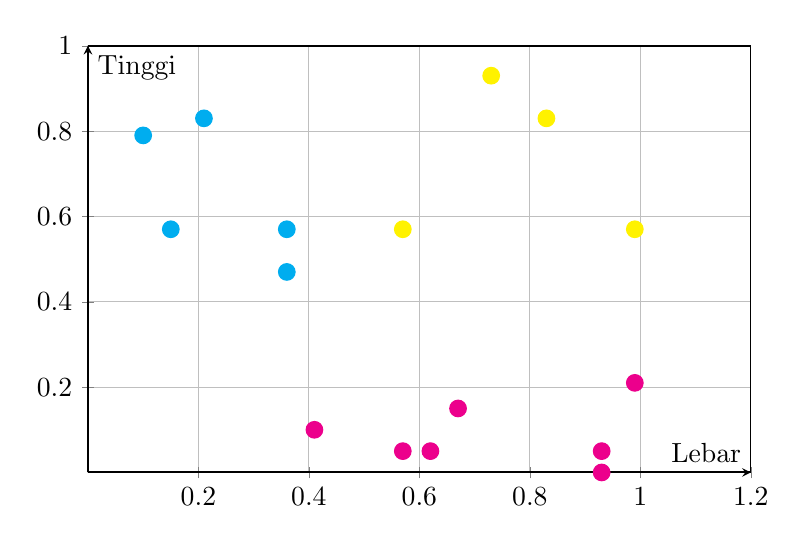
\begin{tikzpicture}
        \begin{axis}[
            xlabel=Lebar,
            ylabel=Tinggi,
            xmin=0, xmax=1.2,
            ymin=0, ymax=1,
            width=10cm,
            height=7cm,
            domain=-4:4,
            grid=both,
            samples=100,
            legend pos=south west,
            axis lines=middle, % Add this line to get the axes in the middle
        ]

        % Adding points
        \addplot[mark=*, color=cyan, mark size = 3] coordinates {(0.36,0.47)};
        \addplot[mark=*, color=cyan, mark size = 3] coordinates {(0.36,0.57)};
        \addplot[mark=*, color=cyan, mark size = 3] coordinates {(0.15,0.57)};
        \addplot[mark=*, color=cyan, mark size = 3] coordinates {(0.10,0.79)};
        \addplot[mark=*, color=cyan, mark size = 3] coordinates {(0.21,0.83)};
        \addplot[mark=*, color=magenta, mark size = 3] coordinates {(0.41,0.10)};
        \addplot[mark=*, color=magenta, mark size = 3] coordinates {(0.62,0.05)};
        \addplot[mark=*, color=magenta, mark size = 3] coordinates {(0.67,0.15)};
        \addplot[mark=*, color=magenta, mark size = 3] coordinates {(0.93,0.00)};
        \addplot[mark=*, color=magenta, mark size = 3] coordinates {(0.93,0.05)};
        \addplot[mark=*, color=magenta, mark size = 3] coordinates {(0.99,0.21)};
        \addplot[mark=*, color=magenta, mark size = 3] coordinates {(0.57,0.05)};
        \addplot[mark=*, color=yellow, mark size = 3] coordinates {(0.83,0.83)};
        \addplot[mark=*, color=yellow, mark size = 3] coordinates {(0.73,0.93)};
        \addplot[mark=*, color=yellow, mark size = 3] coordinates {(0.57,0.57)};
        \addplot[mark=*, color=yellow, mark size = 3] coordinates {(0.99,0.57)};


        % Draw frame
        \draw[black, thick] (rel axis cs:0,0) rectangle (rel axis cs:1,1);
        \end{axis}
    \end{tikzpicture}
    \caption{Grafik dari dataset setelah melalui Minmax Scaling. \textit{Cyan} adalah lemari, \textit{magenta} adalah buffet, dan kuning adalah wardrobe}
    \label{fig:plot dataset normalisasi}
\end{figure}


\subsubsection{Pembuatan \textit{Class Neural Network}}

\begin{figure}[H]
    \centering
    \includegraphics[width=9cm]{contents/chapter-3/Diagram Alir class.drawio.png}
    \caption{Diagram Alir Class Neural Network}
    \label{fig:Flowchart Class}
\end{figure}

Pembuatan \textit{class} ditunjukan agar dengan satu \textit{source code} dapat dilakukan percobaan dengan nilai jaringan tersembunyi yang dapat dirubah-ubah sesuai dengan model yang diinginkan. Pembuatan kelas juga dapat membantu penulis dalam melakukan perbaikan pada program. Diagram alir dari \textit{Class Neural Network} ditunjukkan pada Gambar \ref{fig:Flowchart Class}. 
\begin{lstlisting}
    def __init__(self, input_size, hidden_size, output_size, weight_init=0.5):
        self.input_size = input_size
        self.hidden_size = hidden_size
        self.output_size = output_size
        self.num_layers = np.concatenate(([input_size], hidden_size, [output_size]))
        self.L = len(self.num_layers)-1
        self.weight = {}
        self.Y = {}
        self.F = {}
        self.delta = {}
        self.dJ_dF = {}
        self.dF_dY = {}
        self.dY_dF = {}
        self.dJ_dw = {}
        self.t = 0
        self.d2J_dw2 = {}
        self.accuracy = []
        self.mse = []

        if weight_init == 'random':
            for l in range(0, self.L):
                self.weight[f'w{l}'] = np.random.rand(self.num_layers[l+1], self.num_layers[l]+1)
                self.dJ_dw[f'{l}'] = np.array([])

        else:
            for l in range(0, self.L):
                self.weight[f'w{l}'] = weight_init * np.ones((self.num_layers[l+1], self.num_layers[l]+1))
                self.dJ_dw[f'{l}'] = np.array([])
\end{lstlisting}

Inisialisasi adalah fungsi yang pertama kali dijalankan ketika \textit{Class Neural Network} dipanggil. Inisialisasi akan membuat variabel-variabel yang diperlukan oleh neural network. Termasuk didalamnya adalah bobot awal yang akan digunakan selama pelatihan. Sebagai contoh pada Gambar \ref{fig:2.2 Jaringan Syaraf Tiruan} jaringan tersebut memiliki satu \textit{hidden layer} sehingga jaringan memiliki dua buah bobot maka L akan bernilai 2, bobot tersebut adalah $W^1$ dan $W^2$.

\begin{equation}
    W^1 = 
    \begin{bmatrix}
        W^1_{0,0} & W^1_{0,1} & W^1_{0,2} \\
        W^1_{1,0} & W^1_{1,1} & W^1_{1,2} \\
        W^1_{2,0} & W^1_{2,1} & W^1_{2,2}
    \end{bmatrix}
     W^2 = 
    \begin{bmatrix}
        W^2_{0,0} & W^2_{0,1} & W^2_{0,2} \\
        W^2_{1,0} & W^2_{1,1} & W^2_{1,2} \\
        W^2_{2,0} & W^2_{2,1} & W^2_{2,2}
    \end{bmatrix}
\end{equation}

\begin{equation}
    W^1 = W^2 =  
    \begin{bmatrix}
        1 & 0 & 0 \\
        0.5 & 0.5 & 0.5 \\
        0.5 & 0.5 & 0.5
    \end{bmatrix}
    \label{eq:bobot awal}
\end{equation}

Setelah dibuat variabel untuk bobot maka langkah selanjutnya adalah dengan menentukan nilai bobot awal. Bobot awal ini umumnya dideklarasikan dengan suatu fungsi random. Namun karena fokus pada penelitian ini adalah jumlah dari hidden layer, maka nilai bobot akan dibuat sama, yaitu baris pertama akan bernilai 1 untuk mendistribusikan nilai bias. Kemudian baris lainnya akan bernilai 0.5 sama seperti pada persamaan \ref{eq:bobot awal}. 

\begin{lstlisting}
    def ForwardPropagation(self, X):
        self.X = np.append(np.ones((1, self.N), X, axis = 0)

        for l in range (0, self.L):
            if l == 0 :
                self.Y[f'{l}'] = np.dot(self.weight['w0'], self.X)
                self.F[f'{l}'] = self.tanh(self.Y[f'{l}'])
                self.F[f'{l}'] = np.append(np.ones((1,self.N)), self.F[f'{l}'], axis = 0)
            elif l == len(self.hidden_size):
                self.Y[f'{l}'] = np.dot(self.weight[f'w{l}'], self.F[f'{l-1}'])
                self.F[f'{l}'] = self.tanh(self.Y[f'{l}'])
                self.Y_out = self.Y[f'{l}']
                self.F_out = self.F[f'{l}']
                self.F_step = self.step_function(self.F[f'{l}'])
            else :
                self.Y[f'{l}'] = np.dot(self.weight[f'w{l}'], self.F[f'{l-1}'])
                self.F[f'{l}'] = self.tanh(self.Y[f'{l}'])
                self.F[f'{l}'] = np.append(np.ones((1,self.N)), self.F[f'{l}'], axis = 0)
        return
\end{lstlisting}

Setelah proses inisialisasi selesai dan semua variabel yang diperlukan sudah dibuat. Langkah selanjutnya adalah dengan melakukan \textit{Forward Porpagation} dengan menggunakan Persamaan \ref{eq: 2.8}. Setelah \textit{forward propagation} dilakukan hingga mencapai layer terakhir. Sinyal keluaran pada layer terakhir disebut juga sebagai \textit{predicted value}. \textit{Predicted value} ini bersamaan dengan \textit{expected value} dimasukkan kedalam \textit{loss function} MSE sebagai parameter \textit{error} dari model. Umumnya pada awal pelatihan nilai dari \textit{loss function} akan cukup tinggi. Semakin kecil \textit{loss function} semakin baik pula modelnya. Untuk menurunkan nilai \textit{loss function} dapat menggunakan \textit{Gradient descent} pada persamaan \ref{eq: 2.8}. Yaitu dengan menggunakan turunan \textit{loss function} terhadap parameter yang ingin dilatih. Karena dataset yang digunakan cukup kecil maka seluruh data akan digunakan kedalam data pelatihan. berikut persamaan \ref{eq:fx'} dan \ref{eq:fx''}:

\begin{equation}
    \frac{d\text{MSE}}{dw^l_{(j,i)}}=\frac{d\frac{1}{N} \sum_{n=1}^{N} (d_n-y_n)^2}{dw^l_{(j,i)}}
    \label{eq:fx'}
\end{equation}
\begin{equation}
    \frac{d^2\text{MSE}}{d(w^l_{(j,i)})^2}=\frac{d^2\frac{1}{N} \sum_{n=1}^{N} (d_n-y_n)^2}{d(w^l_{(j,i)})^2}
    \label{eq:fx''}
\end{equation}

Dimana $w^l_{(j,i)}$ adalah bobot ke-l, yang terhubung dengan neuron j dan neuron i, $l=1, 2, ...,L$, $d_n$ adalah \textit{expected value} ke-n atau label ke-n, dan $y_n$ adalah \textit{predicted value} ke-n. Setelah mendapatkan gradiennya dengan Persamaan \ref{eq:fx'} dan Persamaan \ref{eq:fx''} nilai tersebut dimasukkan untuk memperbaharui bobot $w^l_{(j,i)}$. Dengan menggunakan aturan rantai maka penggunaannya diterapkan pada fungsi update seperti berikut :

\begin{lstlisting}
    def update(self, y):
        n = self.X.shape[1]

        for l in range(self.L, -1, -1):
            if l == len(self.hidden_size):
                self.dY_dY[f'{l}'] = self.weight[f'w{l}']
                self.delta[f'{l}'] = (-2 / n)  * (y-self.Y[f'{l}'])
                self.dJ_dw[f'{l}'] = np.dot(self.delta[f'{l}'], self.Y[f'{l-1}'].T)
                temp = self.delta[f'{l}']

                self.d2J_dw2[f'{l}'] = (2 / n) * np.sum(self.Y[f'{l-1}']**2, axis=1)
                self.d2J_dw2[f'{l}'] = np.outer(np.ones(self.output_size), self.d2J_dw2[f'{l}'])
                temp_2 = (2 / n) * np.sum(self.weight[f'w{l}']**2, axis=0)

            elif l == 0:
                self.delta[f'{l}'] = np.dot(self.dY_dY[f'{l+1}'].T, temp)
                self.dJ_dw[f'{l}'] = np.dot(self.delta[f'{l}'], self.X.T)

                self.d2J_dw2[f'{l}'] = np.outer(temp_2[:, np.newaxis], np.sum(self.X**2, axis =1)[np.newaxis, :])

            else:
                self.dY_dY[f'{l}'] = self.weight[f'w{l}']
                self.delta[f'{l}'] = np.dot(self.dY_dY[f'{l+1}'].T, temp)
                self.dJ_dw[f'{l}'] = np.dot(self.delta[f'{l}'], self.Y[f'{l-1}'].T)
                temp = self.delta[f'{l}']

                self.d2J_dw2[f'{l}'] = np.outer(temp_2[:, np.newaxis], np.sum(self.Y[f'{l-1}']**2, axis=1)[np.newaxis, :])
                temp_2 = np.dot(temp_2, self.weight[f'w{l}']**2)

        return
\end{lstlisting}

Setelah mendapatkan \textit{gradient} langkah selanjutnya adalah \textit{backpropagation} yaitu dengan mendistribusikan \textit{gradient} tersebut ke semua bobot yang ada dan melakukan pembaharuan bobot. Pembaharuan bobot menggunakan Persamaan \ref{eq:pembaharuan bobot}. Pembaharuan bobot dilakukan satu persatu yaitu dimulai dengan bobot terdepan yaitu bobot $w^l_{j,i}$. Pelatihan dilakukan pada satu bobot tersebut secara berulang hingga memenuhi kriteria \textit{threshold} pada \textit{relative error}, jika syarat sudah terpenuhi pelatihan pada bobot tersebut berhenti dan dilanjutkan pada bobot selanjutnya. Hal ini dilakukan berulang hingga semua bobot telah dilatih atau jika nilai \textit{predicted value} sudah serupa dengan nilai \textit{expected value}. Penggunaan $i, j,$ dan $l$ untuk memastikan agar semua bobot disetiap layer telah melalui proses pelatihan. Sedangkan $t$ adalah banyak iterasi yang dilakukan karena tiap bobot akan melakukan jumlah pelatihan yang berbeda. $t$ akan digunakan untuk membandingkan waktu komputasi yang dilaksanakan. Penggunaan algoritam tersebut akan disimpan pada fungsi \textit{backpropagation} didalam \textit{class Neural Network} seperti berikut:

\begin{lstlisting}
    def Backpropagation(self, X, y, learning_rate=0.1):
        self.ForwardPropagation(X)
        break_all_loop = False
        for l in range(self.L, -1, -1):
          for j in range(self.num_layers[w+1]):
            for i in range(self.num_layers[w]):
              while True:
                self.update(y)
                self.t +=1

                self.accuracy.append(self.accuracy_func(y, self.F))
                self.mse.append(self.mse_func(y, self.Y_out))

                delta_t = learning_rate * (self.dJ_dw[f'{l}'][j, i]/self.d2J_dw2[f'{l}'][j,i])
                w_n = self.weight[f'w{l}'][j, i] - delta_t

                error = self.error(w_n, self.weight[f'w{l}'][j, i])

                self.weight[f'w{l}'][j, i] = w_n
                self.ForwardPropagation(X)

                if np.sum(np.abs(y-self.F)) == 0:
                  self.accuracy.append(self.accuracy_func(y, self.F))
                  self.mse.append(self.mse_func(y, self.Y_out))
                  break_all_loop = True
                  break
                if error < 0.1 :
                  break

              if break_all_loop == True :
                break
            if break_all_loop == True :
              break
          if break_all_loop == True :
            break

        return
\end{lstlisting}

\subsection{Pengujian program jaringan syaraf tiruan}
Pengujian program jaringan syaraf tiruan dilakukan untuk mengetahui apakah program sudah sesuai dengan perintah yang diharapkan. Salah satu faktor penentu program tersebut telah berjalan dengan baik adalah dengan memperhatikan nilai \textit{loss function}-nya. Pelatihan jaringan syaraf tiruan pada program yang dibuat menggunakan metode \textit{gradient descent}, sehingga nilai dari \textit{loss function} dari program yang benar akan berkurang seiring dengan bertambahnya iterasi pada model tersebut.

\subsection{Pengujian dengan satu hidden layer dengan variasi jumlah neuron}
\begin{lstlisting}
    nn1 = {}
    nn1_mse_iterasi = {}
    nn1_accuracy_iterasi = {}
    for h_n in range (1, 11):
      print(f'Hidden Neuron{h_n}')
      nn1[f'{h_n}'] = NeuralNetwork(2, [h_n], 3, weight_init=0.5)
      nn1[f'{h_n}'].Backpropagation(X, y)
      nn1_mse_iterasi[f'{h_n}'] = []
      nn1_accuracy_iterasi[f'{h_n}'] = []
      for t in range (1, 10000):
        old_mse=nn1[f'{h_n}'].mse[-1]
        nn1_mse_iterasi[f'{h_n}'].append(old_mse)
        nn1_accuracy_iterasi[f'{h_n}'].append(nn1[f'{h_n}'].accuracy[-1])
        nn1[f'{h_n}'].Backpropagation(X, y)
        nn1[f'{h_n}'].ForwardPropagation(X)
        new_mse=nn1[f'{h_n}'].mse[-1]
        if new_mse == old_mse :
          print(f'error epoch ke-{t} :',np.sum((y-nn1[f'{h_n}'].Y_out)**2)/16)
          break
        if t % 100 == 0 :
          print(f'error epoch ke-{t} :',np.sum((y-nn1[f'{h_n}'].Y_out)**2)/16)
        if np.sum(np.abs(y-nn1[f'{h_n}'].F)) == 0:
          nn1_mse_iterasi[f'{h_n}'].append(new_mse)
          nn1_accuracy_iterasi[f'{h_n}'].append(nn1[f'{h_n}'].accuracy[-1])
          print(f'error epoch ke-{t} :',np.sum((y-nn1[f'{h_n}'].Y_out)**2)/16)
          break
\end{lstlisting}

Pada \textit{Source Code} program akan membuat \textit{Class Neural Network} dengan satu hidden layer namun dengan hidden neuron yang bervariasi. Variasi hidden neuron dilakukan dari 1 hingga 10 hidden neuron. Didalam \textit{Source Code} tersebut juga menyimpan beberapa variabel yang akan dianalisis lebih lanjut seperti nilai dari MSE dan juga akurasinya pada iterasi ke $t$.

\subsection{Pengujian dengan variasi jumlah hidden layer dengan jumlah neuron yang sama}

\begin{lstlisting}
    nn_vhl = {}
    nn_vhl_mse_iterasi = {}
    nn_vhl_accuracy_iterasi = {}
    for h_n in range (3, 7):
        start_hidden_layers = 1
        last_hidden_layers = 4
        hidden_neuron = []
        for h_l in range (start_hidden_layers, last_hidden_layers+1):
            print(f'number of hidden layer : {h_l}')
            print(f'number of neuron each hidden layer : {h_n}')
            hidden_neuron.append(h_n)
            nn_vhl[f'{h_n}{h_l}'] = NeuralNetwork(2, hidden_neuron, 3, weight_init= 0.3)
            nn_vhl[f'{h_n}{h_l}'].backward(X, y)
            nn_vhl_mse_iterasi[f'{h_n}{h_l}'] = []
            nn_vhl_accuracy_iterasi[f'{h_n}{h_l}'] = []
            for i in range (10000):
            old_mse = nn_vhl[f'{h_n}{h_l}'].mse[-1]
            nn_vhl_mse_iterasi[f'{h_n}{h_l}'].append(old_mse)
            nn_vhl_accuracy_iterasi[f'{h_n}{h_l}'].append(nn_vhl[f'{h_n}{h_l}'].accuracy[-1])
            nn_vhl[f'{h_n}{h_l}'].backward(X, y, learning_rate=0.1)
            nn_vhl[f'{h_n}{h_l}'].forward(X)
            new_mse = nn_vhl[f'{h_n}{h_l}'].mse[-1]
            nn_vhl[f'{h_n}{h_l}'].backward(X, y, 0.1)
            nn_vhl[f'{h_n}{h_l}'].forward(X)
            if new_mse == old_mse :
              print(f'error epoch ke-{i} :',np.sum((y-nn_vhl[f'{h_n}{h_l}'].Y_out)**2)/16)
              break
            if i % 100 == 0 :
              print(f'error epoch ke-{i} :',np.sum((y-nn_vhl[f'{h_n}{h_l}'].Y_out)**2)/16)
            if np.sum(np.abs(y-nn_vhl[f'{h_n}{h_l}'].F)) == 0:
              nn_vhl_mse_iterasi[f'{h_n}{h_l}'].append(new_mse)
              nn_vhl_accuracy_iterasi[f'{h_n}{h_l}'].append(nn_vhl[f'{h_n}{h_l}'].accuracy[-1])
              print(f'error epoch ke-{i} :',np.sum((y-nn_vhl[f'{h_n}{h_l}'].Y_out)**2)/16)
              break
\end{lstlisting}

Pada pengujian ini yaitu dengan melakukan variasi jumlah hidden layer degan jumlah neuron yang sama pada tiap hidden layernya. variasi jumlah hidden layer dilakukan dari satu hidden layer hingga empat hidden layer. Sedangkan jumlah Hidden Neuron yang dibuat sama dilakukan dari 3 Hidden Neuron hingga 6 Hidden Neuron. Variabel $h\_l$ akan digunakan untuk menyimpan hidden layer yang digunakan. Variabel $h\_n$ digunakan untuk menyimpan jumlah hidden neuron yang digunakan

\subsection{Pengujian dengan variasi jumlah hidden layer dengan jumlah bobot yang sama}

Pada pengujian ini diperlukan jumlah bobot yang sesuai untuk bisa digunakan pada jumlah hidden layer yang bervariasi. Dengan menggunakan faktor-faktor darijumlah bobot yang akan digunakan, ditemukan bobot yang dapat digunakan adalah 72, 105, 144, dan 189.

\begin{lstlisting}
    nn_34643 = NeuralNetwork(2, [4, 6, 4], 3, weight_init=0.3)
    nn_34643_mse_iterasi = []
    nn_34643_accuracy_iterasi = []
    nn_34643.Backpropagation(X, y, learning_rate=0.1)
    for i in range (1, 10000):
      old_mse=nn_34643.mse[-1]
      nn_34643_mse_iterasi.append(old_mse)
      nn_34643_accuracy_iterasi.append(nn_344443.accuracy[-1])
      nn_34643.Backpropagation(X, y, learning_rate=0.1)
      nn_34643.ForwardPropagation(X)
      new_mse = nn_34643.mse[-1]
      if new_mse == old_mse :
        print(f'error epoch ke-{i} :',np.sum((y-nn_34643.Y_out)**2)/16)
        break
      if i % 100 == 0 :
        print(f'error epoch ke-{i} :',np.sum((y-nn_34643.Y_out)**2)/16)
      if np.sum(np.abs(y-nn_34643.F)) == 0:
        nn_34643_mse_iterasi.append(new_mse)
        nn_34643_accuracy_iterasi.append(nn_34643.accuracy[-1])
        print(f'error epoch ke-{i} :',np.sum((y-nn_34643.Y_out)**2)/16)
        break
\end{lstlisting}
Pada \textit{Source Code} diatas menunjukkan bagaimana untuk mencari jumlah bobot yang dapat digunakan. Untuk jumlah bobot sebesar 72 maka arsitektur yang akan dibuat adalah 3-4-6-4-3, 3-6-6-3, dan 3-12-3. Untuk jumlah bobot sebesar 105 maka arsitektur yang akan dibuat adalah 3-5-5-5-5-3 dan 3-7-4-8-3. Untuk jumlah bobot sebesar 144 maka arsitektur yang akan dibuat adalah 3-6-6-6-6-3, 3-3-21-3-3, 3-6-14-3, dan 3-24-3, Untuk jumlah bobot sebesar 72 maka arsitektur yang akan dibuat adalah 3-7-7-7-7-3, 3-10-6-11-3, dan 3-6-19-3. Dengan Kombinasi tersebut maka akan dihasilkan jumlah bobot yang sama.

\subsection{Pengambilan data}
Setelah program sudah diyakini benar maka langkah selanjutnya adalah mengambil data yang ingin dianalisis. Dalam penelitian ini data yang diambil adalah jumlah \textit{hidden layer}, akurasi, dan waktu komputasi.